\documentclass{beamer}

% Frame Number
\setbeamertemplate{footline}[frame number]

% Input Encoding
\usepackage[utf8]{inputenc}

% PDF Bookmarks
\usepackage{url}
\usepackage{hyperref} 
\hypersetup{colorlinks}
\hypersetup{bookmarksopen}
\hypersetup{bookmarksnumbered}
\hypersetup{citecolor=blue}
\hypersetup{urlcolor=blue}
\hypersetup{linkcolor=blue}

% Spacing
\usepackage{xspace}

% Figures
\usepackage{graphicx}
\graphicspath{{../../img/}}
\usepackage{subcaption}

% Tables
\usepackage{booktabs}

% Strike Through
\usepackage{ulem}

% Code Snippet 
\usepackage{listings}
\lstset{
  belowcaptionskip=1\baselineskip,
  breaklines=true,
  frame=L,
  xleftmargin=\parindent,
  numbers=left,
  stepnumber=2,
  language=C,
  tabsize=2,
  showstringspaces=false,
  basicstyle=\footnotesize\ttfamily,
  keywordstyle=\bfseries\color{blue},
  commentstyle=\itshape\color{gray},
  identifierstyle=\bfseries\color{black},
  stringstyle=\bfseries\color{purple},
}

% Title
\title[Nanvix]{%
	\textbf{%
		The Nanvix Operating System\\
		\small{Process Scheduling}
	}
}

% Authors
\author[Pedro H. Penna]{%
	Pedro H. Penna%
}

% Affiliations
\institute{
	\url{pedrohenriquepenna@gmail.com}
}

% Short-Hands
\newcommand{\ie}{\textit{ie.\xspace}}

\begin{document}

\frame{\titlepage}

\section{Background on Process Scheduling}

	\begin{frame}
	\frametitle{Background Process Scheduling}
	\framesubtitle{Barebones}
		\begin{itemize}
		\setlength\itemsep{1.5em}
			\item Process compete for processor time	
			\item Process scheduler chooses which process to run
		\end{itemize}
		\begin{figure}
			\centering
			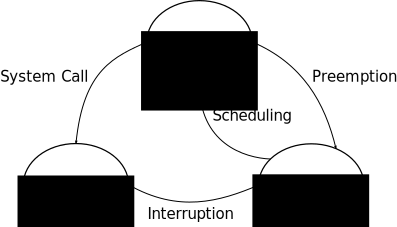
\includegraphics[width=0.6\linewidth]{states}	
			\caption{Process states.}
		\end{figure}
	\end{frame}

	\begin{frame}
	\frametitle{Background on Process Scheduling}
	\framesubtitle{Rules of Thumb}
		\begin{itemize}
		\setlength\itemsep{1.5em}
			\uncover<1->{
				\item All systems	
				\begin{itemize}
				\setlength\itemsep{0.5em}
					\item Fairness
					\item Policy enforcement
					\item Load balancing
				\end{itemize}
			}
			\uncover<2->{
				\item Batch systems
				\begin{itemize}	
				\setlength\itemsep{0.5em}
					\item Throughput
					\item Turnaround time
				\end{itemize}
			}
			\uncover<3->{
				\item Interactive systems
				\begin{itemize}	
				\setlength\itemsep{0.5em}
					\item Response time
					\item Proportionality
				\end{itemize}
			}
		\end{itemize}
	\end{frame}
	
	\begin{frame}
	\frametitle{Background on Process Scheduling}
	\framesubtitle{Classical Algorithms}
		\begin{itemize}
		\setlength\itemsep{1.5em}
			\uncover<1->{
				\item Batch systems
				\begin{itemize}
				\setlength\itemsep{0.5em}
					\item First-Come First-Served
					\item Shortest-Job First
					\item Shortest Remaining Time Next
				\end{itemize}
			}
			\uncover<2->{
				\item Interactive systems
				\begin{itemize}
				\setlength\itemsep{0.5em}
					\item Round-Robin Scheduling
					\item Priority Scheduling
					\item Multiple Queues Scheduling
					\item Lottery Scheduling
					\item Fair-Share Scheduling
				\end{itemize}
			}
		\end{itemize}
	\end{frame}

\section{Process Scheduling in Nanvix}

	\begin{frame}
	\frametitle{Process Scheduling in Nanvix}
	\framesubtitle{Process States}
		\begin{figure}
			\centering
			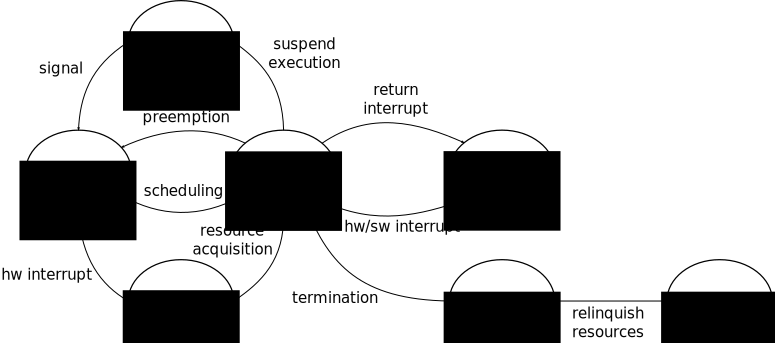
\includegraphics[width=\linewidth]{nanvix-states}
			\caption{States of a process in Nanvix.}
		\end{figure}
	\end{frame}

	\begin{frame}
	\frametitle{Process Scheduling in Nanvix}
	\framesubtitle{Current Implementation}
		\begin{itemize}
		\setlength\itemsep{1.0em}
			\uncover<1->{
				\item Process table entry -- \texttt{struct process}
				\begin{itemize}
				\setlength\itemsep{0.5em}
					\item \texttt{include/nanvix/pm.h}
				\end{itemize}
			}
			\uncover<2->{
				\item Process scheduler -- \texttt{yield()}
				\begin{itemize}
				\setlength\itemsep{0.5em}
					\item \texttt{src/kernel/pm/sched.c}
				\end{itemize}
			}
			\uncover<3->{
				\item Round-robin scheduling
				\begin{itemize}
				\setlength\itemsep{0.5em}
					\item Schedule ready process that is waiting longer 
					\item Give each process a same processor quantum
				\end{itemize}
			}
			\uncover<4->{
				\item Support for priority scheduling (unused)
				\begin{itemize}
				\setlength\itemsep{0.5em}
					\item Static priority (\texttt{priority})
					\item Dynamic priority (\texttt{counter})
					\item User priority (\texttt{nice})
				\end{itemize}
			}
		\end{itemize}
	\end{frame}

\end{document}
